%% LyX 2.2.3 created this file.  For more info, see http://www.lyx.org/.
%% Do not edit unless you really know what you are doing.
\documentclass[english]{beamer}
\usepackage[latin9]{inputenc}
\setcounter{secnumdepth}{3}
\setcounter{tocdepth}{3}
\usepackage{refstyle}
\usepackage{graphicx}

\makeatletter

%%%%%%%%%%%%%%%%%%%%%%%%%%%%%% LyX specific LaTeX commands.
\RS@ifundefined{subsecref}
  {\newref{subsec}{name = \RSsectxt}}
  {}
\RS@ifundefined{thmref}
  {\def\RSthmtxt{theorem~}\newref{thm}{name = \RSthmtxt}}
  {}
\RS@ifundefined{lemref}
  {\def\RSlemtxt{lemma~}\newref{lem}{name = \RSlemtxt}}
  {}


%%%%%%%%%%%%%%%%%%%%%%%%%%%%%% Textclass specific LaTeX commands.
 % this default might be overridden by plain title style
 \newcommand\makebeamertitle{\frame{\maketitle}}%
 % (ERT) argument for the TOC
 \AtBeginDocument{%
   \let\origtableofcontents=\tableofcontents
   \def\tableofcontents{\@ifnextchar[{\origtableofcontents}{\gobbletableofcontents}}
   \def\gobbletableofcontents#1{\origtableofcontents}
 }

\makeatother

\usepackage{babel}
\begin{document}

\title{Optimal enforcement of non-competes}

\author{Nicolas Fernandez-Arias}
\makebeamertitle
\begin{frame}{Motivation}
\begin{itemize}
\item A non-compete is part of an employment contract that restricts an
employee from working for a competitor for a certain amount of time
after leaving their current employer (usually 1-2 years)
\begin{itemize}
\item Protect IP (NDAs hard to enforce)
\item Restrict flow of knowledge
\item and many other effects... (e.g. worker bargaining power, market concentration,
incentives for human capital accumulation)
\end{itemize}
\item Very prevalent
\begin{itemize}
\item 70\% of senior executives (Garmaise 2011)
\item Nearly 50\% of engineers (Marx 2011)
\end{itemize}
\end{itemize}
\end{frame}
%
\begin{frame}{Motivation}
\begin{itemize}
\item Differing enforcement regimes across U.S. states \ref{mapofenforcement}
\begin{itemize}
\item Emerging consensus that Silicon Valley, CA displaced Rt. 128, MA as
high-tech hub due to non-enforcement (Saxenian 1994, Gilson 1999,
etc.)
\item Oct 2016 - Obama administration ``call to action'' to state legislatures
to reduce enforcement of non-competes
\item 11 state legislatures currently considering weakening enforcement;
some Federal laws already passed
\end{itemize}
\end{itemize}
\end{frame}
%

\begin{itemize}
\item Non-enforcing regimes
\begin{itemize}
\item Grow more in response to exogenous increases in supply of VC funding
(Samila-Sorenson 2011)
\item Have more mobile workforces (Fallick et al. 2006, Garmaise 2011, Marx
et. al 2009)
\item Make small firms more able to compete with large firms, leading to
less market concentration (Kang-Fleming 2017)
\item Employees have better lifetime wage profiles (Chang et al. 2017)
\end{itemize}
\end{itemize}
\end{frame}
%
\begin{frame}{Theoretical work}
\begin{itemize}
\item Paper showing reallocation from enforcing to non-enforcing in second
period, consistent with SV vs. Rt 128 story (citation)
\item Some theory showing potential advantages of not having non-competes
\begin{itemize}
\item Allows for reallocation of skilled labor when uncertainty about firm
``experiments'' is resolved
\end{itemize}
\item Not difficult to write a model in which non-competes make knowledge
worth nothing \textendash \textgreater{} no growth
\item So all depends on parameters and stength of different mechanisms
\end{itemize}
\end{frame}
%
\begin{frame}{Optimal enforcement}
\begin{itemize}
\item Empirical evidence seems to suggest optimal not to enforce
\begin{itemize}
\item Contrary to intuition about the benefit of having free contracts
\end{itemize}
\item Theoretical work has less clear conclusions 
\item But what about spillovers?
\begin{itemize}
\item Most charitably: non-enforcing states ``do better'' than enforcing
states, and states ``do better'' when they exogenously switch from
enforcement to non-enforcement
\item ``Crowding out'' story: brain drain to non-enforcing regimes after
exogenous shift to enforcing regime (Marx 2015)
\end{itemize}
\item How to rule out this explanation?
\begin{itemize}
\item Even with exogenous changes, no ``control'' for the entire USA
\item Need a (well-calibrated) model of the aggregate economy 
\item Welfare analysis
\end{itemize}
\end{itemize}
\end{frame}
%
\begin{frame}{Methodology}
\begin{itemize}
\item For now:
\begin{itemize}
\item Klette \& Kortum 2004 style model endogenizing knowledge spillovers
via workers leaving incumbents to start rival startups
\item Non-enforcement leads to faster knowledge spillovers, but reduces
value of knowledge, disincentivizing R\&D (c.f. Arrow 1962)
\item Goal: calibrate using LEHD, Crunchbase, LinkedIn data
\item Test model by seeing extent to which it can reproduce cross-sectional
empirical results in the data
\item Counterfactual productivity growth and welfare analysis
\end{itemize}
\item Future work: 
\begin{itemize}
\item Multiple incumbents competing over workers 
\item Worker human capital accumulation
\item Endogenous contracting (for now, simply assume that non-competes are
used in enforcing regimes)
\end{itemize}
\end{itemize}
\end{frame}
%
\begin{frame}{Enforcement}
\label{mapofenforcement}

\begin{figure}
\caption{Map of enforcement across US states}

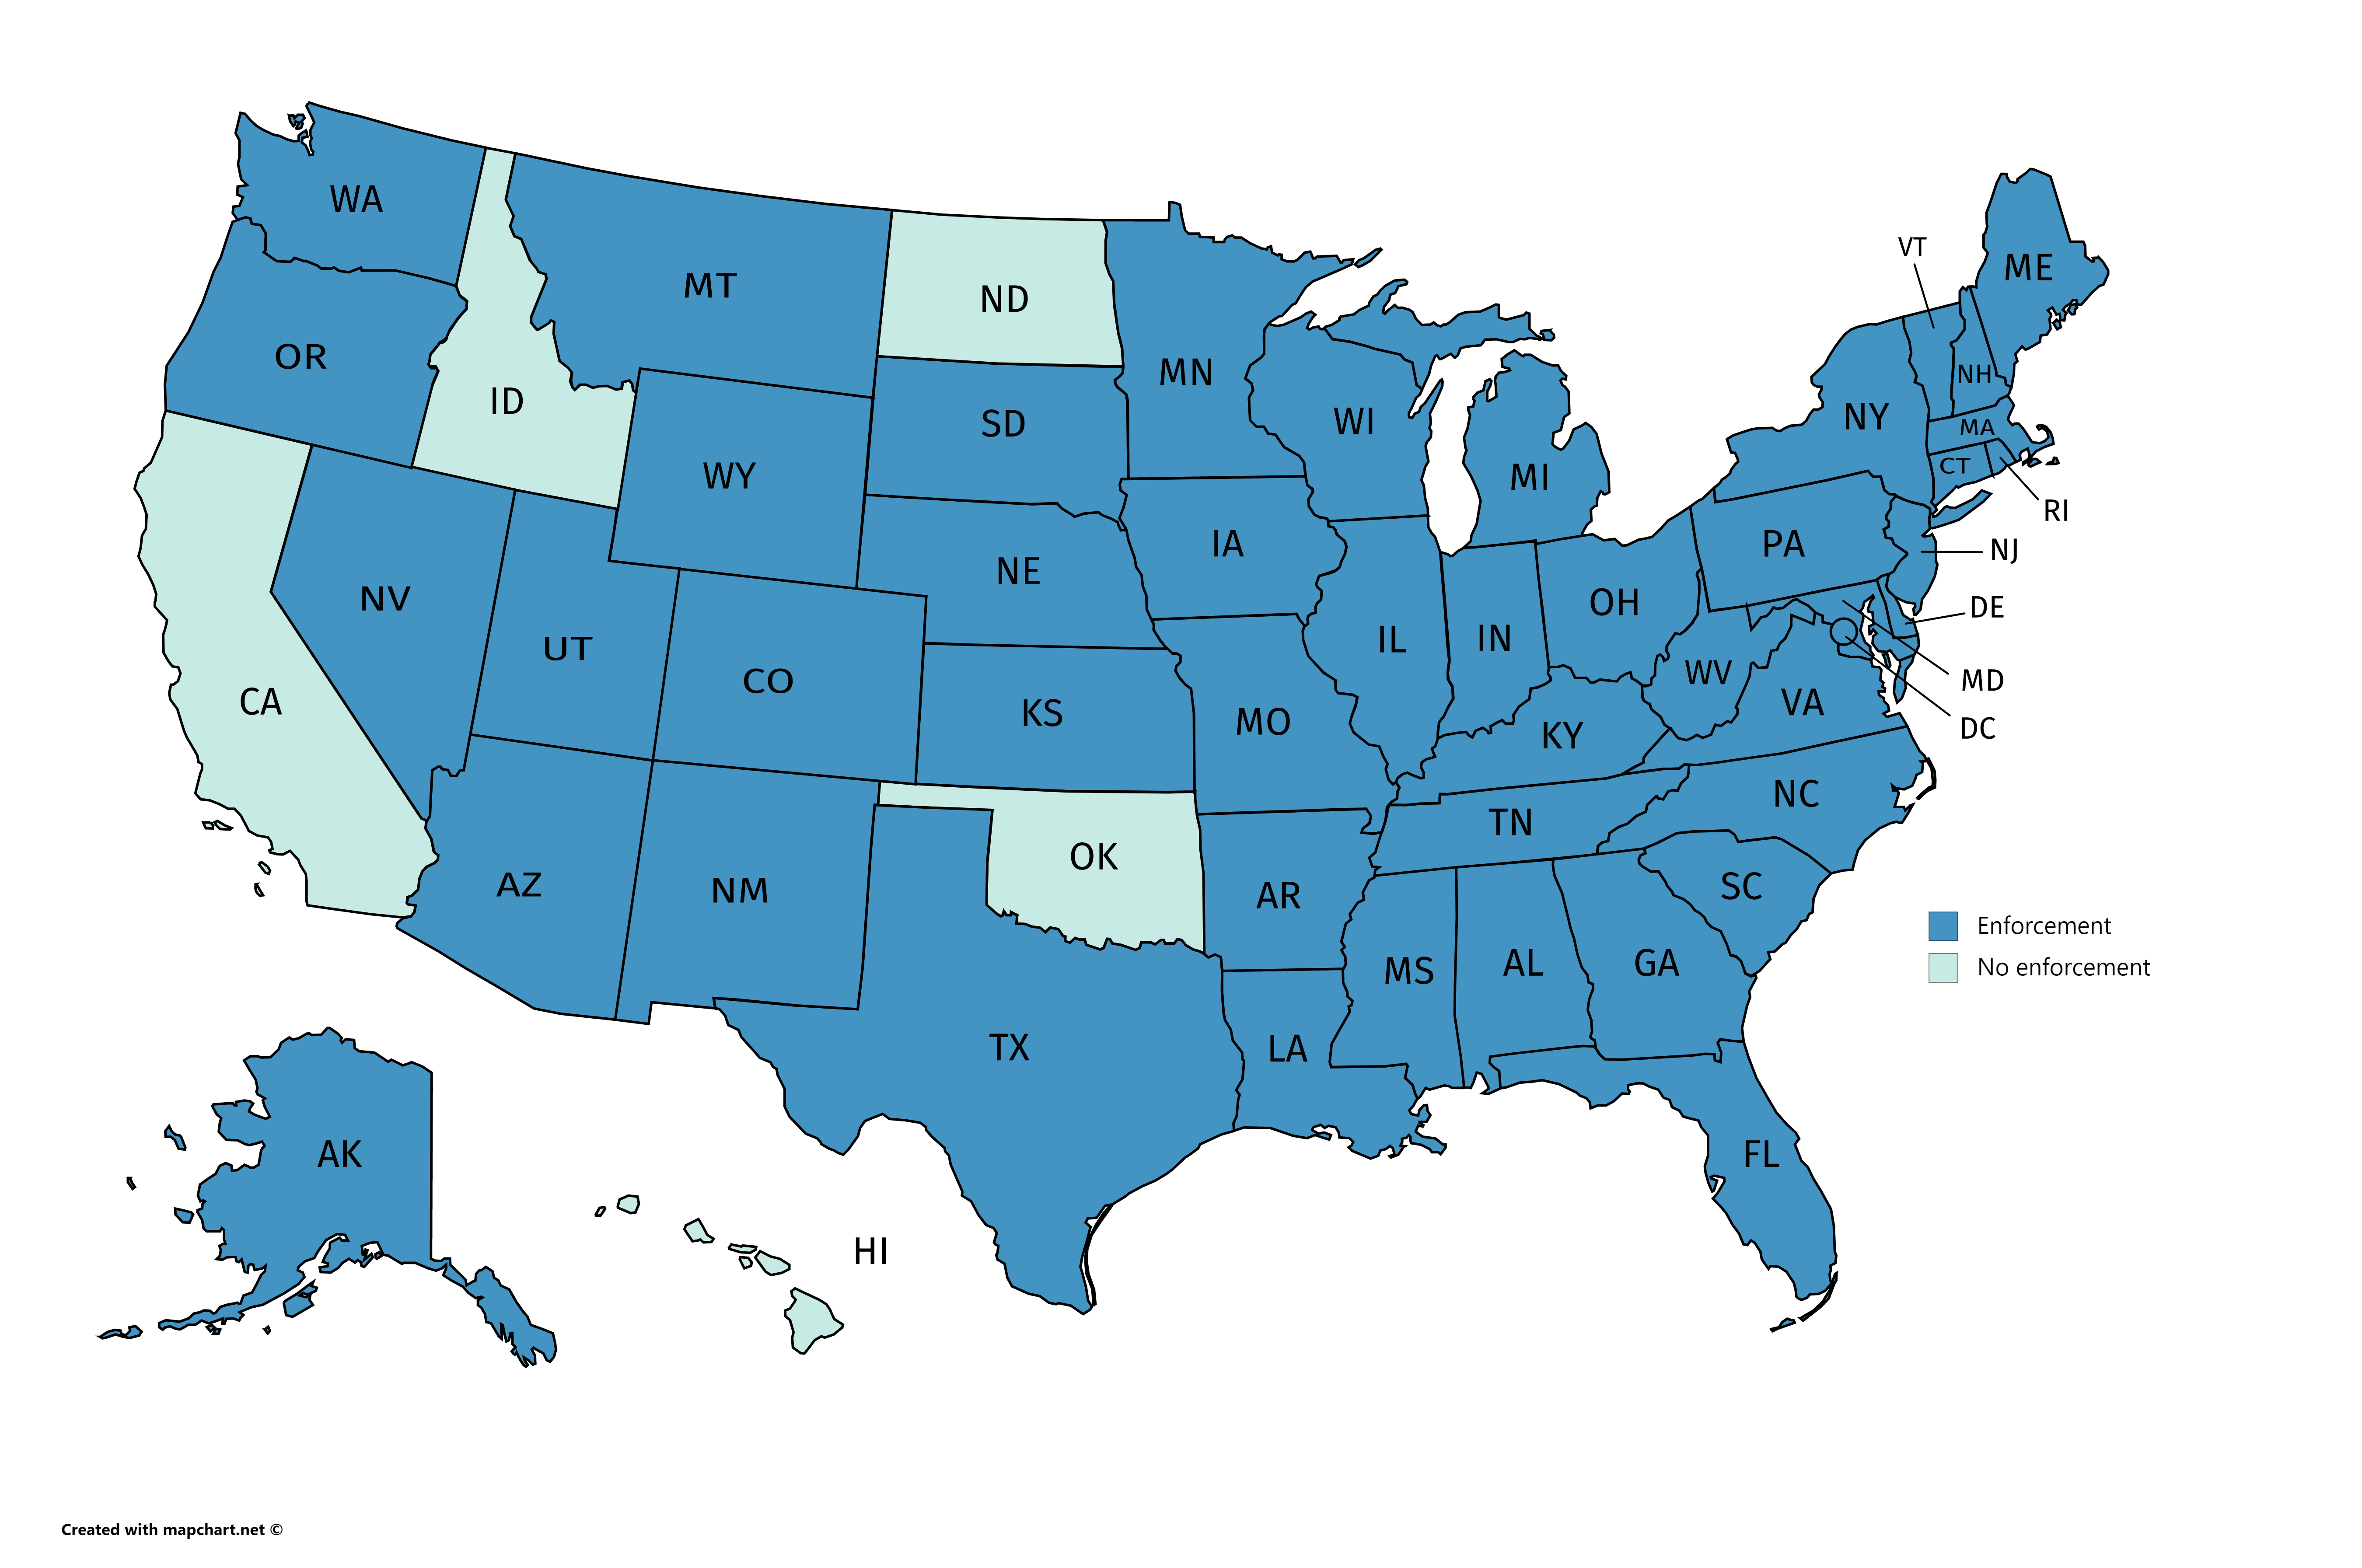
\includegraphics[scale=0.05]{figures/map_of_enforcement}

\end{figure}
\end{frame}

\end{document}
